\documentclass[]{book}
\usepackage{lmodern}
\usepackage{amssymb,amsmath}
\usepackage{ifxetex,ifluatex}
\usepackage{fixltx2e} % provides \textsubscript
\ifnum 0\ifxetex 1\fi\ifluatex 1\fi=0 % if pdftex
  \usepackage[T1]{fontenc}
  \usepackage[utf8]{inputenc}
\else % if luatex or xelatex
  \ifxetex
    \usepackage{mathspec}
  \else
    \usepackage{fontspec}
  \fi
  \defaultfontfeatures{Ligatures=TeX,Scale=MatchLowercase}
\fi
% use upquote if available, for straight quotes in verbatim environments
\IfFileExists{upquote.sty}{\usepackage{upquote}}{}
% use microtype if available
\IfFileExists{microtype.sty}{%
\usepackage{microtype}
\UseMicrotypeSet[protrusion]{basicmath} % disable protrusion for tt fonts
}{}
\usepackage[margin=1in]{geometry}
\usepackage{hyperref}
\hypersetup{unicode=true,
            pdftitle={Validation Report for adoptr package},
            pdfauthor={Kevin Kunzmann \& Maximilian Pilz},
            pdfborder={0 0 0},
            breaklinks=true}
\urlstyle{same}  % don't use monospace font for urls
\usepackage{natbib}
\bibliographystyle{apalike}
\usepackage{color}
\usepackage{fancyvrb}
\newcommand{\VerbBar}{|}
\newcommand{\VERB}{\Verb[commandchars=\\\{\}]}
\DefineVerbatimEnvironment{Highlighting}{Verbatim}{commandchars=\\\{\}}
% Add ',fontsize=\small' for more characters per line
\usepackage{framed}
\definecolor{shadecolor}{RGB}{248,248,248}
\newenvironment{Shaded}{\begin{snugshade}}{\end{snugshade}}
\newcommand{\AlertTok}[1]{\textcolor[rgb]{0.94,0.16,0.16}{#1}}
\newcommand{\AnnotationTok}[1]{\textcolor[rgb]{0.56,0.35,0.01}{\textbf{\textit{#1}}}}
\newcommand{\AttributeTok}[1]{\textcolor[rgb]{0.77,0.63,0.00}{#1}}
\newcommand{\BaseNTok}[1]{\textcolor[rgb]{0.00,0.00,0.81}{#1}}
\newcommand{\BuiltInTok}[1]{#1}
\newcommand{\CharTok}[1]{\textcolor[rgb]{0.31,0.60,0.02}{#1}}
\newcommand{\CommentTok}[1]{\textcolor[rgb]{0.56,0.35,0.01}{\textit{#1}}}
\newcommand{\CommentVarTok}[1]{\textcolor[rgb]{0.56,0.35,0.01}{\textbf{\textit{#1}}}}
\newcommand{\ConstantTok}[1]{\textcolor[rgb]{0.00,0.00,0.00}{#1}}
\newcommand{\ControlFlowTok}[1]{\textcolor[rgb]{0.13,0.29,0.53}{\textbf{#1}}}
\newcommand{\DataTypeTok}[1]{\textcolor[rgb]{0.13,0.29,0.53}{#1}}
\newcommand{\DecValTok}[1]{\textcolor[rgb]{0.00,0.00,0.81}{#1}}
\newcommand{\DocumentationTok}[1]{\textcolor[rgb]{0.56,0.35,0.01}{\textbf{\textit{#1}}}}
\newcommand{\ErrorTok}[1]{\textcolor[rgb]{0.64,0.00,0.00}{\textbf{#1}}}
\newcommand{\ExtensionTok}[1]{#1}
\newcommand{\FloatTok}[1]{\textcolor[rgb]{0.00,0.00,0.81}{#1}}
\newcommand{\FunctionTok}[1]{\textcolor[rgb]{0.00,0.00,0.00}{#1}}
\newcommand{\ImportTok}[1]{#1}
\newcommand{\InformationTok}[1]{\textcolor[rgb]{0.56,0.35,0.01}{\textbf{\textit{#1}}}}
\newcommand{\KeywordTok}[1]{\textcolor[rgb]{0.13,0.29,0.53}{\textbf{#1}}}
\newcommand{\NormalTok}[1]{#1}
\newcommand{\OperatorTok}[1]{\textcolor[rgb]{0.81,0.36,0.00}{\textbf{#1}}}
\newcommand{\OtherTok}[1]{\textcolor[rgb]{0.56,0.35,0.01}{#1}}
\newcommand{\PreprocessorTok}[1]{\textcolor[rgb]{0.56,0.35,0.01}{\textit{#1}}}
\newcommand{\RegionMarkerTok}[1]{#1}
\newcommand{\SpecialCharTok}[1]{\textcolor[rgb]{0.00,0.00,0.00}{#1}}
\newcommand{\SpecialStringTok}[1]{\textcolor[rgb]{0.31,0.60,0.02}{#1}}
\newcommand{\StringTok}[1]{\textcolor[rgb]{0.31,0.60,0.02}{#1}}
\newcommand{\VariableTok}[1]{\textcolor[rgb]{0.00,0.00,0.00}{#1}}
\newcommand{\VerbatimStringTok}[1]{\textcolor[rgb]{0.31,0.60,0.02}{#1}}
\newcommand{\WarningTok}[1]{\textcolor[rgb]{0.56,0.35,0.01}{\textbf{\textit{#1}}}}
\usepackage{longtable,booktabs}
\usepackage{graphicx,grffile}
\makeatletter
\def\maxwidth{\ifdim\Gin@nat@width>\linewidth\linewidth\else\Gin@nat@width\fi}
\def\maxheight{\ifdim\Gin@nat@height>\textheight\textheight\else\Gin@nat@height\fi}
\makeatother
% Scale images if necessary, so that they will not overflow the page
% margins by default, and it is still possible to overwrite the defaults
% using explicit options in \includegraphics[width, height, ...]{}
\setkeys{Gin}{width=\maxwidth,height=\maxheight,keepaspectratio}
\IfFileExists{parskip.sty}{%
\usepackage{parskip}
}{% else
\setlength{\parindent}{0pt}
\setlength{\parskip}{6pt plus 2pt minus 1pt}
}
\setlength{\emergencystretch}{3em}  % prevent overfull lines
\providecommand{\tightlist}{%
  \setlength{\itemsep}{0pt}\setlength{\parskip}{0pt}}
\setcounter{secnumdepth}{5}
% Redefines (sub)paragraphs to behave more like sections
\ifx\paragraph\undefined\else
\let\oldparagraph\paragraph
\renewcommand{\paragraph}[1]{\oldparagraph{#1}\mbox{}}
\fi
\ifx\subparagraph\undefined\else
\let\oldsubparagraph\subparagraph
\renewcommand{\subparagraph}[1]{\oldsubparagraph{#1}\mbox{}}
\fi

%%% Use protect on footnotes to avoid problems with footnotes in titles
\let\rmarkdownfootnote\footnote%
\def\footnote{\protect\rmarkdownfootnote}

%%% Change title format to be more compact
\usepackage{titling}

% Create subtitle command for use in maketitle
\providecommand{\subtitle}[1]{
  \posttitle{
    \begin{center}\large#1\end{center}
    }
}

\setlength{\droptitle}{-2em}

  \title{Validation Report for \textbf{adoptr} package}
    \pretitle{\vspace{\droptitle}\centering\huge}
  \posttitle{\par}
    \author{Kevin Kunzmann \& Maximilian Pilz}
    \preauthor{\centering\large\emph}
  \postauthor{\par}
      \predate{\centering\large\emph}
  \postdate{\par}
    \date{2019-03-31}

\usepackage{booktabs}

\begin{document}
\maketitle

{
\setcounter{tocdepth}{1}
\tableofcontents
}
\hypertarget{introduction}{%
\chapter{Introduction}\label{introduction}}

\hypertarget{concept}{%
\section{Concept}\label{concept}}

The goal of adoptrValidation is to provide a comprehensive suit of test
for the \href{https://github.com/kkmann/adoptr}{adoptr} package.
The package is not directly inteded to be used but to automatically
deploy a weekly validation report via github pages to
\url{https://kkmann.github.io/adoptrValidation/}.
The report is implemented as a set of vignettes which are compiled
into a static web page using pkgdown.
For details on the class of supported designs, see
\url{https://github.com/kkmann/adoptr}.

\hypertarget{local-validation}{%
\section{Local validation}\label{local-validation}}

\ldots{}

\hypertarget{brief-introdcution-to-two-stage-designs}{%
\section{Brief Introdcution to Two-Stage Designs}\label{brief-introdcution-to-two-stage-designs}}

In \texttt{adoptrValidation} a suitable set of cases is tested in order to
validate the performance of the package \texttt{adoptr}.
This package allows to compute optimal designs (adaptive two-stage,
group-sequential two-stage and one-stage) for normally distributed data.
For a treatment group \(T\) and a control group \(C\) where
the observations \(X_i^T \sim \mathcal{N} (\mu_T, \sigma^2)\),
\(X_i^C \sim \mathcal{N} (\mu_C, \sigma^2)\) the following hypotheses are
tested:
\[
\mathcal{H}_0: \delta := \mu_T - \mu_C \leq 0 \text{ v.s. }
\mathcal{H_1}: \delta > 0. 
\]
The power of a test procedure is computed on an alternative effect size
\(\delta_1 > 0\) where a prior distribution
\(\delta_1 \sim \pi(\vartheta, \tau^2)\) is imaginable.

The trial evaluation happens as follows.
After \(n_1\) patients (per group) finished the trial an interim analysis
is conducted. The interim test statistic \(Z_1\) for a standard z-test is computed
and the trial is stopped early for futility, if \(Z_1 < c_f\).
If \(Z_1 > c_e\) the null hypothesis is rejected and the trial is stopped early
for efficacy. Otherwise, i.e.~if \(c_f \leq Z_1 \leq c_e\), the trial enters
in the second stage. Due to the adaptivness of the trial design, the
stage-two sample size is a function of \(Z_1\), i.e. \(n_2(Z_1)\).
Also the final rejection boundary \(c_2\) depends on \(Z_1\).
At the final analysis the stage-two test statistic \(Z_2\) is computed and
the null hypothesis is rejected if \(Z_2 > c_2(Z_1)\).

A design \(D\) is a five-tuple consisting of the first-stage sample size
\(n_1\), early stopping boundaries \(c_f\) (futility) and \(c_e\) (efficacy)
and stage-two functions \(n_2(\cdot)\) (sample size) and \(c_2(\cdot)\)
(rejection boundary).
All these elements can be computed optimally in \texttt{adoptr}.
The incorporation of continuous priors is possible as well as including
conditional and unconditional constraints.

Given a design \(D\) and a objective function \(f\)
the default setting in {[}adoptr{]} is the following.

\begin{longtable}[]{@{}ll@{}}
\toprule
\(\min\) & \(f(D)\)\tabularnewline
\midrule
\endhead
such that & Type One Error Rate \(\leq \alpha\)\tabularnewline
and & Power \(\geq 1 - \beta\)\tabularnewline
\bottomrule
\end{longtable}

Often in clinical practice one is not willing to enter in a second
stage when the conditional power (i.e., the probability to reject at
the final analysis given the first-stage results) is too low or too high
because in these cases the stage-two result is likely predictable.
Therefore, introducing conditional power constraints of the form
\[
1 - \beta_2 \leq \text{Conditional Power}(z_1, D) \leq 1 - \beta_3
\]
may be desirable and are supported by \texttt{adoptr}.

In \texttt{adoptrValidation} different scenarios are investigated.
Each scenario is determined by the assumed effect size \(\delta_1\) and its
prior distribution \(\pi\).
In each scenario, different tests are performed.
All tests are indicated by a bullet point.

\hypertarget{validation-strategy}{%
\section{Validation strategy}\label{validation-strategy}}

\textbf{adoptrValidation} essentially extends the test suit of \textbf{adoptr} to cover
more different scenarios.
In order to generate a proper validation report the test Variants are not managed
using a unit testing framework like testthat but are directly included in a
set of vignettes (one per sceanrio).
These vignettes are automatically built and published (here) once per week
using pkgdown to keep the validation report up to date with the latest
CRAN release {[}TODO: we currently use our master!{]}.
The overall failure/pass status of the latest build can be checked using the
Travis-CI badge.
In the following, all Scenarios and their respective sub-Variants are outlined.
\textbf{Scenarios} are defined by the joint distribution of the test statistic and the
location parameter, while \textbf{Variants} are given by the respective optimization
problem (objective, constraints).

\hypertarget{technical-setup}{%
\subsection{Technical Setup}\label{technical-setup}}

Initially, the both packages are loaded and the seed for simulation is set.
Additionally, the options for optimization are modified by increasing
the maximum number of evaluations to ensure convergence.

\begin{Shaded}
\begin{Highlighting}[]
\KeywordTok{library}\NormalTok{(adoptr)}
\KeywordTok{library}\NormalTok{(tidyverse)}

\CommentTok{# load custom functions in folder subfolder '/R'}
\ControlFlowTok{for}\NormalTok{ (nm }\ControlFlowTok{in} \KeywordTok{list.files}\NormalTok{(}\StringTok{"R"}\NormalTok{, }\DataTypeTok{pattern =} \StringTok{"}\CharTok{\textbackslash{}\textbackslash{}}\StringTok{.[RrSsQq]$"}\NormalTok{))}
   \KeywordTok{source}\NormalTok{(}\KeywordTok{file.path}\NormalTok{(}\StringTok{"R"}\NormalTok{, nm))}

\CommentTok{# define seed value}
\NormalTok{seed <-}\StringTok{ }\DecValTok{42}

\CommentTok{# define custom tolerance and iteration limit for nloptr}
\NormalTok{opts =}\StringTok{ }\KeywordTok{list}\NormalTok{(}
    \DataTypeTok{algorithm =} \StringTok{"NLOPT_LN_COBYLA"}\NormalTok{,}
    \DataTypeTok{xtol_rel  =} \FloatTok{1e-5}\NormalTok{,}
    \DataTypeTok{maxeval   =} \DecValTok{50000}
\NormalTok{)}
\end{Highlighting}
\end{Shaded}

\hypertarget{scenario-i}{%
\subsection{\texorpdfstring{\href{https://kkmann.github.io/adoptrValidation/articles/scenario-I.html\#tocnav}{Scenario I}}{Scenario I}}\label{scenario-i}}

This is the default scenario.

\begin{itemize}
\tightlist
\item
  \textbf{Data distribution:} Two-armed trial with normally distributed test statistic
\item
  \textbf{Prior:} \(\delta\sim\delta_{0.4}\)
\item
  \textbf{Null hypothesis:} \(\mathcal{H}_0:\delta \leq 0\)
\end{itemize}

\hypertarget{variant-i.1-minimizing-expected-sample-size-under-the-alternative}{%
\subsubsection{\texorpdfstring{\href{https://kkmann.github.io/adoptrValidation/articles/scenario-I.html\#case-i-1-minimizing-expected-sample-size-under-point-prior}{Variant I.1: Minimizing Expected Sample Size under the Alternative}}{Variant I.1: Minimizing Expected Sample Size under the Alternative}}\label{variant-i.1-minimizing-expected-sample-size-under-the-alternative}}

\begin{itemize}
\tightlist
\item
  \textbf{Objective:} \(ESS := \boldsymbol{E}\big[n(X_1)\,|\,\delta=0.4\big]\)
\item
  \textbf{Constraints:}

  \begin{enumerate}
  \def\labelenumi{\arabic{enumi}.}
  \tightlist
  \item
    \(Power := \boldsymbol{Pr}\big[c_2(X_1) < X_2\,|\,\delta=0.4\big] \geq 0.8\)
  \item
    \(TOER := \boldsymbol{Pr}\big[c_2(X_1) < X_2\,|\,\delta=0.0\big] \leq 0.025\)
  \item
    Three variants: two-stage, group-sequential, one-stage.
  \end{enumerate}
\item
  \textbf{Formal tests:}

  \begin{enumerate}
  \def\labelenumi{\arabic{enumi}.}
  \tightlist
  \item
    All three \textbf{adoptr} variants (two-stage, group-sequential, one-stage)
    comply with constraints. Internally validated by testing vs.~simulated
    values of the power curve at respective points.
  \item
    \(ESS\) of optimal two-stage design is lower than \(ESS\) of optimal
    group-sequential one and that is in turn lower than the one of the
    optimal one-stage design.
  \item
    \(ESS\) of optimal group-sequential design is lower than \(ESS\) of
    externally computed group-sequential design using the \href{https://rpact.org/}{rpact} package.
  \item
    Are the \(ESS\) values obtained from simulation the same as the ones
    obtained by using numerical integration via \texttt{adoptr::evaluate}?
  \item
    Is \(n()\) of the optimal two-stage design monotonously decreasing on
    continuation area?
  \end{enumerate}
\end{itemize}

\hypertarget{variant-i.2-minimizing-expected-sample-size-under-the-null-hypothesis}{%
\subsubsection{\texorpdfstring{\href{https://kkmann.github.io/adoptrValidation/articles/scenario-I.html\#case-i-2-minimizing-expected-sample-size-under-null-hypothesis}{Variant I.2: Minimizing Expected Sample Size under the Null Hypothesis}}{Variant I.2: Minimizing Expected Sample Size under the Null Hypothesis}}\label{variant-i.2-minimizing-expected-sample-size-under-the-null-hypothesis}}

\begin{itemize}
\tightlist
\item
  \textbf{Objective:} \(ESS := \boldsymbol{E}\big[n(X_1)\,|\,\color{red}{\delta=0.0}\big]\)
\item
  \textbf{Constraints:}

  \begin{enumerate}
  \def\labelenumi{\arabic{enumi}.}
  \tightlist
  \item
    \(Power := \boldsymbol{Pr}\big[c_2(X_1) < X_2\,|\,\delta=0.4\big] \geq 0.8\)
  \item
    \(TOER := \boldsymbol{Pr}\big[c_2(X_1) < X_2\,|\,\delta=0.0\big] \leq 0.025\)
  \end{enumerate}
\item
  \textbf{Formal tests:}

  \begin{enumerate}
  \def\labelenumi{\arabic{enumi}.}
  \tightlist
  \item
    Validate constraint compliance by testing vs.~simulated
    values of the power curve at respective points.
  \item
    \(n()\) of optimal design is monotonously increasing on continuation area.
    TODO
  \item
    \(ESS\) of optimal two-stage design is lower than \(ESS\) of externally
    computed group-sequential design using the \href{https://rpact.org/}{rpact} package.
  \item
    Are the \(ESS\) values obtained from simulation the same as the ones
    obtained by using numerical integration via \texttt{adoptr::evaluate}?
  \end{enumerate}
\end{itemize}

\hypertarget{variant-i.3-condtional-power-constraint}{%
\subsubsection{\texorpdfstring{\href{https://kkmann.github.io/adoptrValidation/articles/scenario-I.html\#case-i-3-conditional-power-constraint}{Variant I.3: Condtional Power Constraint}}{Variant I.3: Condtional Power Constraint}}\label{variant-i.3-condtional-power-constraint}}

\begin{itemize}
\tightlist
\item
  \textbf{Objective:} \(ESS := \boldsymbol{E}\big[n(X_1)\,|\,\delta=0.4\big]\)
\item
  \textbf{Constraints:}

  \begin{enumerate}
  \def\labelenumi{\arabic{enumi}.}
  \tightlist
  \item
    \(Power := \boldsymbol{Pr}\big[c_2(X_1) < X_2\,|\,\delta=0.4\big] \geq 0.8\)
  \item
    \(TOER := \boldsymbol{Pr}\big[c_2(X_1) < X_2\,|\,\delta=0.0\big] \leq 0.025\)
  \item
    \(CP := \color{red}{\boldsymbol{Pr}\big[c_2(X_1) < X_2\,|\,\delta=0.4, X_1 = x_1\big] \geq 0.7}\) for all \(x_1\in(c_1^f, c_1^e)\)
  \end{enumerate}
\item
  \textbf{Formal tests:}

  \begin{enumerate}
  \def\labelenumi{\arabic{enumi}.}
  \tightlist
  \item
    Check \(Power\) and \(TOER\) constraints with simulation.
    Check \(CP\) constraint on three different values of \(x_1\) in
    \((c_1^f, c_1^e)\)
  \item
    Are the \(CP\) values at the three test-pivots obtained from simulation the
    same as the ones obtained by using numerical integration via
    \texttt{adoptr::evaluate}?
  \item
    Is \(ESS\) of optimal two-stage design with \(CP\) constraint higher than
    \(ESS\) of optimal two-stage design without this constraint?
  \end{enumerate}
\end{itemize}

\hypertarget{scenario-ii}{%
\subsection{\texorpdfstring{\href{https://kkmann.github.io/adoptrValidation/articles/scenario-II.html\#tocnav}{Scenario II}}{Scenario II}}\label{scenario-ii}}

Similar in scope to Scenario I, but with a continuous Gaussian prior on \(\delta\).

\begin{itemize}
\tightlist
\item
  \textbf{Data distribution:} Two-armed trial with normally distributed test statistic
\item
  \textbf{Prior:} \(\delta\sim\mathcal{N}(0.4, .3)\)
\item
  \textbf{Null hypothesis:} \(\mathcal{H}_0:\delta \leq 0\)
\end{itemize}

\hypertarget{variant-ii.1-minimizing-expected-sample-size}{%
\subsubsection{\texorpdfstring{\href{https://kkmann.github.io/adoptrValidation/articles/scenario-II.html\#case-ii-1-minimizing-expected-sample-size-under-point-prior}{Variant II.1: Minimizing Expected Sample Size}}{Variant II.1: Minimizing Expected Sample Size}}\label{variant-ii.1-minimizing-expected-sample-size}}

\begin{itemize}
\tightlist
\item
  \textbf{Objective:} \(ESS := \boldsymbol{E}\big[n(X_1)\big]\)
\item
  \textbf{Constraints:}

  \begin{enumerate}
  \def\labelenumi{\arabic{enumi}.}
  \tightlist
  \item
    \(Power := \boldsymbol{Pr}\big[c_2(X_1) < X_2\,|\,\delta> 0.0\big] \geq 0.8\)
  \item
    \(TOER := \boldsymbol{Pr}\big[c_2(X_1) < X_2\,|\,\delta=0.0\big] \leq 0.025\)
  \item
    Three variants: two-stage, group-sequential, one-stage.
  \end{enumerate}
\item
  \textbf{Formal tests:}

  \begin{enumerate}
  \def\labelenumi{\arabic{enumi}.}
  \tightlist
  \item
    All designs comply with type one error rate constraints (tested via
    simulation).
  \item
    \(ESS\) of optimal two-stage design is lower than \(ESS\) of optimal
    group-sequential one and that is in turn lower than the one of the
    optimal one-stage design.
  \end{enumerate}
\end{itemize}

\hypertarget{variant-ii.2-minimizing-expected-sample-size-under-the-null-hypothesis}{%
\subsubsection{\texorpdfstring{\href{https://kkmann.github.io/adoptrValidation/articles/scenario-II.html\#case-ii-2-minimizing-expected-sample-size-under-null-hypothesis}{Variant II.2: Minimizing Expected Sample Size under the Null hypothesis}}{Variant II.2: Minimizing Expected Sample Size under the Null hypothesis}}\label{variant-ii.2-minimizing-expected-sample-size-under-the-null-hypothesis}}

\begin{itemize}
\tightlist
\item
  \textbf{Objective:} \(ESS := \boldsymbol{E}\big[n(X_1)\,|\,\color{red}{\delta\leq 0}\big]\)
\item
  \textbf{Constraints:}

  \begin{enumerate}
  \def\labelenumi{\arabic{enumi}.}
  \tightlist
  \item
    \(Power := \boldsymbol{Pr}\big[c_2(X_1) < X_2\,|\,\delta> 0.0\big] \geq 0.8\)
  \item
    \(TOER := \boldsymbol{Pr}\big[c_2(X_1) < X_2\,|\,\delta=0.0\big] \leq 0.025\)
  \end{enumerate}
\item
  \textbf{Formal tests:}

  \begin{enumerate}
  \def\labelenumi{\arabic{enumi}.}
  \tightlist
  \item
    Does the design comply with \(TOER\) constraint (via simulation)?
  \item
    Check \(CP\) constraint on three different values of \(x_1\) in
    \((c_1^f, c_1^e)\)
  \item
    TODO: Is the sample size function monotonously increasing?
  \item
    Is \(ESS\) lower than expected sample size under the null hypothesis
    for the optimal two stage design from Variant II-1?
  \end{enumerate}
\end{itemize}

\hypertarget{variant-ii.3-condtional-power-constraint}{%
\subsubsection{\texorpdfstring{\href{https://kkmann.github.io/adoptrValidation/articles/scenario-II.html\#case-ii-3-conditional-power-constraint}{Variant II.3: Condtional Power Constraint}}{Variant II.3: Condtional Power Constraint}}\label{variant-ii.3-condtional-power-constraint}}

\begin{itemize}
\tightlist
\item
  \textbf{Objective:} \(ESS := \boldsymbol{E}\big[n(X_1)\big]\)
\item
  \textbf{Constraints:}

  \begin{enumerate}
  \def\labelenumi{\arabic{enumi}.}
  \tightlist
  \item
    \(Power := \boldsymbol{Pr}\big[c_2(X_1) < X_2\,|\,\delta>0.0\big] \geq 0.8\)
  \item
    \(TOER := \boldsymbol{Pr}\big[c_2(X_1) < X_2\,|\,\delta=0.0\big] \leq 0.025\)
  \item
    \(CP := \color{red}{\boldsymbol{Pr}\big[c_2(X_1) < X_2\,|\,\delta> 0.0, X_1 = x_1\big] \geq 0.7}\)
    for all \(x_1\in(c_1^f, c_1^e)\)
  \end{enumerate}
\item
  \textbf{Formal tests:}

  \begin{enumerate}
  \def\labelenumi{\arabic{enumi}.}
  \tightlist
  \item
    Check \(TOER\) constraint with simulation.
    Check \(CP\) constraint on three different values of \(x_1\) in
    \((c_1^f, c_1^e)\)
  \item
    Is \(ESS\) of optimal two-stage design with \(CP\) constraint higher than
    \(ESS\) of optimal two-stage design without the constraint?
  \end{enumerate}
\end{itemize}

\hypertarget{scenario-iii}{%
\subsection{\texorpdfstring{\href{https://kkmann.github.io/adoptrValidation/articles/scenario-III.html\#tocnav}{Scenario III:}}{Scenario III:}}\label{scenario-iii}}

\begin{itemize}
\tightlist
\item
  \textbf{Data distribution:} Two-armed trial with normally distributed test statistic
\item
  \textbf{Prior:} sequence of uniform distributions
  \(\delta\sim\operatorname{Unif}(0.4 - \Delta_i, 0.4 + \Delta_i)\)
  around \(0.4\) with \(\Delta_i=(3 - i)/10\) for \(i=0\ldots 3\).
  I.e., for \(\Delta_3=0\) reduces to a point prior on \(\delta=0.4\).
\item
  \textbf{Null hypothesis:} \(\mathcal{H}_0:\delta \leq 0\)
\end{itemize}

\hypertarget{variant-iii.1-convergence-under-prior-concentration}{%
\subsubsection{\texorpdfstring{\href{https://kkmann.github.io/adoptrValidation/articles/scenario-III.html\#Variant-iii-1-minimizing-expected-sample-size-under-alternative}{Variant III.1: Convergence under Prior Concentration}}{Variant III.1: Convergence under Prior Concentration}}\label{variant-iii.1-convergence-under-prior-concentration}}

\begin{itemize}
\tightlist
\item
  \textbf{Objective:} \(ESS := \boldsymbol{E}\big[n(X_1)\big]\)
\item
  \textbf{Constraints:}

  \begin{enumerate}
  \def\labelenumi{\arabic{enumi}.}
  \tightlist
  \item
    \(Power := \boldsymbol{Pr}\big[c_2(X_1) < X_2\,|\,\delta>0.0\big] \geq 0.8\)
  \item
    \(TOER := \boldsymbol{Pr}\big[c_2(X_1) < X_2\,|\,\delta=0.0\big] \leq 0.025\)
  \end{enumerate}
\item
  \textbf{Formal tests:}

  \begin{enumerate}
  \def\labelenumi{\arabic{enumi}.}
  \tightlist
  \item
    Simulated type one error rate is compared to \(TOER\) constraint for each
    design.
  \item
    Number of iterations are checked agaist default maximum to ensure proper
    convergence.
  \item
    TODO: \(ESS\) decreases with prior variance.
  \end{enumerate}
\end{itemize}

Additionally, the designs are compared graphically.
Inspect the plot to see convergence pattern.

\hypertarget{scenario-iv-smaller-effect-size-larger-trials.}{%
\subsection{\texorpdfstring{\href{https://kkmann.github.io/adoptrValidation/articles/scenario-IV.html\#tocnav}{Scenario IV: Smaller effect size, larger trials.}}{Scenario IV: Smaller effect size, larger trials.}}\label{scenario-iv-smaller-effect-size-larger-trials.}}

\hypertarget{variant-iv.1-minimizing-expected-sample-size-under-the-alternative}{%
\subsubsection{\texorpdfstring{\href{https://kkmann.github.io/adoptrValidation/articles/scenario-IV.html\#Variant-iv-1-minimizing-expected-sample-size-under-alternative}{Variant IV.1: Minimizing Expected Sample Size under the Alternative}}{Variant IV.1: Minimizing Expected Sample Size under the Alternative}}\label{variant-iv.1-minimizing-expected-sample-size-under-the-alternative}}

\begin{itemize}
\tightlist
\item
  \textbf{Objective:} \(ESS := \boldsymbol{E}\big[n(X_1)\,|\,\delta=0.2\big]\)
\item
  \textbf{Constraints:}

  \begin{enumerate}
  \def\labelenumi{\arabic{enumi}.}
  \tightlist
  \item
    \(Power := \boldsymbol{Pr}\big[c_2(X_1) < X_2\,|\,\delta=0.2\big] \geq 0.8\)
  \item
    \(TOER := \boldsymbol{Pr}\big[c_2(X_1) < X_2\,|\,\delta=0.0\big] \leq 0.025\)
  \item
    Three variants: two-stage, group-sequential, one-stage.
  \end{enumerate}
\item
  \textbf{Formal tests:}

  \begin{enumerate}
  \def\labelenumi{\arabic{enumi}.}
  \tightlist
  \item
    All three adoptr variants (two-stage, group-sequential, one-stage)
    comply with costraints. Internally validated by testing vs.~simulated
    values of the power curve at respective points.
  \item
    \(ESS\) of optimal two-stage design is lower than \(ESS\) of optimal
    group-sequential one and that is in tunr lower than the one of the
    optimal one-stage design.
  \item
    \(ESS\) of optimal group-sequential design is lower than \(ESS\) of
    externally computed group-sequential design using the \href{https://rpact.org/}{rpact} package.
  \item
    Are the \(ESS\) values obtained from simulation the same as the ones
    obtained by using numerical integration via \texttt{adoptr::evaluate}?
  \item
    Is \(n()\) of the optimal two-stage design monotonously decreasing on
    continuation area? TODO
  \end{enumerate}
\end{itemize}

\hypertarget{variant-iv.2-increasing-power}{%
\subsubsection{\texorpdfstring{\href{https://kkmann.github.io/adoptrValidation/articles/scenario-IV.html\#Variant-iv-2-increase-power}{Variant IV.2: Increasing Power}}{Variant IV.2: Increasing Power}}\label{variant-iv.2-increasing-power}}

\begin{itemize}
\tightlist
\item
  \textbf{Objective:} \(ESS := \boldsymbol{E}\big[n(X_1)\,|\,\delta=0.2\big]\)
\item
  \textbf{Constraints:}

  \begin{enumerate}
  \def\labelenumi{\arabic{enumi}.}
  \tightlist
  \item
    \(Power := \boldsymbol{Pr}\big[c_2(X_1) < X_2\,|\,\delta=0.2\big] \geq \color{red}{0.9}\)
  \item
    \(TOER := \boldsymbol{Pr}\big[c_2(X_1) < X_2\,|\,\delta=0.0\big] \leq 0.025\)
  \item
    Three variants: two-stage, group-sequential, one-stage.
  \end{enumerate}
\item
  \textbf{Formal tests:}

  \begin{enumerate}
  \def\labelenumi{\arabic{enumi}.}
  \tightlist
  \item
    Does the design respect all constraints (via simulation)?
  \item
    \(ESS\) of optimal two-stage design is lower than \(ESS\) of optimal
    group-sequential one and that is in tunr lower than the one of the
    optimal one-stage design.
  \item
    \(ESS\) of optimal group-sequential design is lower than \(ESS\) of
    externally computed group-sequential design using the \href{https://rpact.org/}{rpact} package.
  \item
    Are the \(ESS\) values obtained from simulation the same as the ones
    obtained by using numerical integration via \texttt{adoptr::evaluate}?
  \item
    Is \(n()\) of the optimal two-stage design monotonously decreasing on
    continuation area? TODO
  \end{enumerate}
\end{itemize}

\hypertarget{variant-iv.3-increasing-maximal-type-one-error-rate}{%
\subsubsection{\texorpdfstring{\href{https://kkmann.github.io/adoptrValidation/articles/scenario-IV.html\#Variant-iv-3-increase-maximal-type-one-error-rate}{Variant IV.3: Increasing Maximal Type One Error Rate}}{Variant IV.3: Increasing Maximal Type One Error Rate}}\label{variant-iv.3-increasing-maximal-type-one-error-rate}}

\begin{itemize}
\tightlist
\item
  \textbf{Objective:} \(ESS := \boldsymbol{E}\big[n(X_1)\,|\,\delta=0.2\big]\)
\item
  \textbf{Constraints:}

  \begin{enumerate}
  \def\labelenumi{\arabic{enumi}.}
  \tightlist
  \item
    \(Power := \boldsymbol{Pr}\big[c_2(X_1) < X_2\,|\,\delta=0.2\big] \geq 0.8\)
  \item
    \(TOER := \boldsymbol{Pr}\big[c_2(X_1) < X_2\,|\,\delta=0.0\big] \leq \color{red}{0.05}\)
  \item
    Three variants: two-stage, group-sequential, one-stage.
  \end{enumerate}
\item
  \textbf{Formal tests:}

  \begin{enumerate}
  \def\labelenumi{\arabic{enumi}.}
  \tightlist
  \item
    Does the design respect all constraints (via simulation)?
  \item
    \(ESS\) of optimal two-stage design is lower than \(ESS\) of optimal
    group-sequential one and that is in tunr lower than the one of the
    optimal one-stage design.
  \item
    \(ESS\) of optimal group-sequential design is lower than \(ESS\) of
    externally computed group-sequential design using the \href{https://rpact.org/}{rpact} package.
  \item
    Are the \(ESS\) values obtained from simulation the same as the ones
    obtained by using numerical integration via \texttt{adoptr::evaluate}?
  \item
    Is \(n()\) of the optimal two-stage design monotonously decreasing on
    continuation area? TODO
  \end{enumerate}
\end{itemize}

\hypertarget{scenario-v-single-arm-design-medium-effect-size.}{%
\subsection{\texorpdfstring{\href{https://kkmann.github.io/adoptrValidation/articles/scenario-V.html\#tocnav}{Scenario V: Single-arm design, medium effect size.}}{Scenario V: Single-arm design, medium effect size.}}\label{scenario-v-single-arm-design-medium-effect-size.}}

\begin{itemize}
\tightlist
\item
  \textbf{Data distribution:} One-armed trial with normally distributed test statistic
\item
  \textbf{Prior:} \(\delta\sim\delta_{0.3}\)
\item
  \textbf{Null hypothesis:} \(\mathcal{H}_0:\delta \leq 0\)
\end{itemize}

\hypertarget{variant-v.1-sensitivity-to-integration-order}{%
\subsubsection{\texorpdfstring{\href{https://kkmann.github.io/adoptrValidation/articles/scenario-V.html\#case-v-1-sensitivity-to-integration-order}{Variant V.1: Sensitivity to Integration Order}}{Variant V.1: Sensitivity to Integration Order}}\label{variant-v.1-sensitivity-to-integration-order}}

\begin{itemize}
\tightlist
\item
  \textbf{Objective:} \(ESS := \boldsymbol{E}\big[n(X_1)\,|\,\delta=0.3\big]\)
\item
  \textbf{Constraints:}

  \begin{enumerate}
  \def\labelenumi{\arabic{enumi}.}
  \tightlist
  \item
    \(Power := \boldsymbol{Pr}\big[c_2(X_1) < X_2\,|\,\color{red}{\delta=0.3}\big] \geq 0.8\)
  \item
    \(TOER := \boldsymbol{Pr}\big[c_2(X_1) < X_2\,|\,\delta=0.0\big] \leq 0.025\)
  \item
    Three variants: integration order 5, 8, 11 two-stage designs {[}TODO: maybe more?{]}.
  \end{enumerate}
\item
  \textbf{Formal tests:}

  \begin{enumerate}
  \def\labelenumi{\arabic{enumi}.}
  \tightlist
  \item
    Do all designs respect all constraints (via simulation)?
  \item
    Do all designs converge within the respective iteration limit?
  \item
    Does constraint compliance get better with increased order?
  \item
    Does the simulated \(ESS\) get better with increased order?
  \end{enumerate}
\end{itemize}

\hypertarget{variant-v.2-utility-maximization}{%
\subsubsection{\texorpdfstring{\href{https://kkmann.github.io/adoptrValidation/articles/scenario-V.html\#case-v-2-utility-maximization}{Variant V.2: Utility Maximization}}{Variant V.2: Utility Maximization}}\label{variant-v.2-utility-maximization}}

\begin{itemize}
\tightlist
\item
  \textbf{Objective:} \(\lambda\, Power - ESS := \lambda\, \boldsymbol{Pr}\big[c_2(X_1) < X_2\,|\,\delta=0.3\big] - \boldsymbol{E}\big[n(X_1)\,|\,\delta=0.3\big].\)
  for \(\lambda = 100\) and \(200\)
\item
  \textbf{Constraints:}

  \begin{enumerate}
  \def\labelenumi{\arabic{enumi}.}
  \tightlist
  \item
    \(TOER := \boldsymbol{Pr}\big[c_2(X_1) < X_2\,|\,\delta=0.0\big] \leq 0.025\)
  \end{enumerate}
\item
  \textbf{Formal tests:}

  \begin{enumerate}
  \def\labelenumi{\arabic{enumi}.}
  \tightlist
  \item
    Do both desings respect the type one error rate constraint (via simulation)?
  \item
    Is the power of the design with larger \(\lambda\) larger?
  \end{enumerate}
\end{itemize}

\hypertarget{variant-v.3-n_1-penalty}{%
\subsubsection{\texorpdfstring{\href{https://kkmann.github.io/adoptrValidation/articles/scenario-V.html\#case-v-3-n1-penalty}{Variant V.3: \(n_1\) penalty}}{Variant V.3: n\_1 penalty}}\label{variant-v.3-n_1-penalty}}

\begin{itemize}
\tightlist
\item
  \textbf{Objective:} \(ESS := \boldsymbol{E}\big[n(X_1)\,|\,\delta=0.3\big] + \lambda \, n_1\)
  for \(\lambda = 0.05\) and \(0.2\).
\item
  \textbf{Constraints:}

  \begin{enumerate}
  \def\labelenumi{\arabic{enumi}.}
  \tightlist
  \item
    \(TOER := \boldsymbol{Pr}\big[c_2(X_1) < X_2\,|\,\delta=0.0\big] \leq 0.025\)
  \item
    \(Power := \boldsymbol{Pr}\big[c_2(X_1) < X_2\,|\,\delta=0.3\big] \geq 0.8\)
  \end{enumerate}
\item
  \textbf{Formal tests:}

  \begin{enumerate}
  \def\labelenumi{\arabic{enumi}.}
  \tightlist
  \item
    Is \(n_1\) for the optimal design smaller than the order-5 design in V.1?
  \end{enumerate}
\end{itemize}

\hypertarget{variant-v.4-n_2-penalty}{%
\subsubsection{\texorpdfstring{\href{https://kkmann.github.io/adoptrValidation/articles/scenario-V.html\#case-v-4-n2-penalty}{Variant V.4: \(n_2\) penalty}}{Variant V.4: n\_2 penalty}}\label{variant-v.4-n_2-penalty}}

\begin{itemize}
\tightlist
\item
  \textbf{Objective:} \(ESS := \boldsymbol{E}\big[n(X_1)\,|\,\delta=0.3\big] +\) \texttt{AverageN2}
\item
  \textbf{Constraints:}

  \begin{enumerate}
  \def\labelenumi{\arabic{enumi}.}
  \tightlist
  \item
    \(TOER := \boldsymbol{Pr}\big[c_2(X_1) < X_2\,|\,\delta=0.0\big] \leq 0.025\)
  \item
    \(Power := \boldsymbol{Pr}\big[c_2(X_1) < X_2\,|\,\delta=0.3\big] \geq 0.8\)
  \end{enumerate}
\item
  \textbf{Formal tests:}

  \begin{enumerate}
  \def\labelenumi{\arabic{enumi}.}
  \tightlist
  \item
    Is the \texttt{AverageN2} for the optimal design smaller than for the order-5
    design in V.1?
  \end{enumerate}
\end{itemize}

\hypertarget{scenario-i-large-effect-point-alternative}{%
\chapter{Scenario I: large effect, point alternative}\label{scenario-i-large-effect-point-alternative}}

\hypertarget{details}{%
\section{Details}\label{details}}

In this scenario an alternative effect size of \(\delta = 0.4\) with
point prior distribution is investigated.
The null hypothesis is \(\delta \leq 0\).
Currently, \texttt{adoptr} only supports normal distributed data what is widely spread
in the development of adaptive designs.
We protect the one-sided type one error rate at \(\alpha = 0.025\) and require
the power of the design to be at least \(1 - \beta = 0.8\).

\hypertarget{data-distribution}{%
\subsection{Data distribution}\label{data-distribution}}

Two-armed trial with normally distributed test statistic

\begin{Shaded}
\begin{Highlighting}[]
\NormalTok{datadist <-}\StringTok{ }\KeywordTok{Normal}\NormalTok{(}\DataTypeTok{two_armed =} \OtherTok{TRUE}\NormalTok{)}
\end{Highlighting}
\end{Shaded}

\hypertarget{null-hypothesis}{%
\subsection{Null hypothesis}\label{null-hypothesis}}

The null hypothesis is \(\mathcal{H}_0:\delta \leq 0\)

\begin{Shaded}
\begin{Highlighting}[]
\NormalTok{H_}\DecValTok{0}\NormalTok{ <-}\StringTok{ }\KeywordTok{PointMassPrior}\NormalTok{(.}\DecValTok{0}\NormalTok{, }\DecValTok{1}\NormalTok{)}
\end{Highlighting}
\end{Shaded}

\hypertarget{prior-assumptions}{%
\subsection{Prior assumptions}\label{prior-assumptions}}

A point mass prior with probability mass on \(\delta = 0.4\) is assumed.

\begin{Shaded}
\begin{Highlighting}[]
\NormalTok{prior <-}\StringTok{ }\KeywordTok{PointMassPrior}\NormalTok{(.}\DecValTok{4}\NormalTok{, }\DecValTok{1}\NormalTok{)}
\end{Highlighting}
\end{Shaded}

\hypertarget{case-i-1-minimizing-expected-sample-size-under-point-prior}{%
\section{Case I-1: Minimizing Expected Sample Size under Point Prior}\label{case-i-1-minimizing-expected-sample-size-under-point-prior}}

\hypertarget{objective}{%
\subsection{Objective}\label{objective}}

Expected sample size under the respective prior is minimized, i.e.,
\(\boldsymbol{E}\big[n(\mathcal{D})\big]\).

\begin{Shaded}
\begin{Highlighting}[]
\NormalTok{ess <-}\StringTok{ }\KeywordTok{expected}\NormalTok{(}\KeywordTok{ConditionalSampleSize}\NormalTok{(datadist, prior))}
\end{Highlighting}
\end{Shaded}

\hypertarget{constrains}{%
\subsection{Constrains}\label{constrains}}

The type one error rate is controlled at \(0.025\) on the boundary of the
null hypothesis.

\begin{Shaded}
\begin{Highlighting}[]
\NormalTok{toer_cnstr <-}\StringTok{ }\KeywordTok{expected}\NormalTok{(}\KeywordTok{ConditionalPower}\NormalTok{(datadist, H_}\DecValTok{0}\NormalTok{)) }\OperatorTok{<=}\StringTok{ }\FloatTok{.025}
\end{Highlighting}
\end{Shaded}

Power must be larger than \(0.8\).

\begin{Shaded}
\begin{Highlighting}[]
\NormalTok{pow_cnstr <-}\StringTok{ }\KeywordTok{expected}\NormalTok{(}\KeywordTok{ConditionalPower}\NormalTok{(datadist, prior)) }\OperatorTok{>=}\StringTok{ }\FloatTok{.8}
\end{Highlighting}
\end{Shaded}

\hypertarget{initial-design}{%
\subsection{Initial Design}\label{initial-design}}

\texttt{adoptr} requires the definition of an initial design for optimization.
We start with a group-sequential design from the package \texttt{rpact} that
fulfills these constraints and is used later for comparison.
The order of integration is set to

\begin{Shaded}
\begin{Highlighting}[]
\NormalTok{order <-}\StringTok{ }\NormalTok{7L}
\end{Highlighting}
\end{Shaded}

For usage as two-stage design with variable sample size, it has to
be converted to a \texttt{TwoStageDesign}.

\begin{Shaded}
\begin{Highlighting}[]
\NormalTok{init_design_gs <-}\StringTok{ }\KeywordTok{rpact_design}\NormalTok{(}\FloatTok{0.4}\NormalTok{, }\FloatTok{0.025}\NormalTok{, }\FloatTok{0.8}\NormalTok{, }\OtherTok{TRUE}\NormalTok{, order)}

\NormalTok{init_design    <-}\StringTok{ }\KeywordTok{TwoStageDesign}\NormalTok{(init_design_gs)}
\end{Highlighting}
\end{Shaded}

\hypertarget{optimization}{%
\subsection{Optimization}\label{optimization}}

The optimal design is computed in three variants: two-stage, group-sequential
and one-stage.
The input only differs with regard to the initial design.

\begin{Shaded}
\begin{Highlighting}[]
\NormalTok{opt_design <-}\StringTok{ }\ControlFlowTok{function}\NormalTok{(initial_design) \{}
    \KeywordTok{minimize}\NormalTok{(}
        
\NormalTok{        ess,}
        
        \KeywordTok{subject_to}\NormalTok{(}
            
\NormalTok{            toer_cnstr,}
\NormalTok{            pow_cnstr}
            
\NormalTok{        ),}
        
        \DataTypeTok{initial_design =}\NormalTok{ initial_design,}
        
        \DataTypeTok{opts =}\NormalTok{ opts}
        
\NormalTok{    )}
\NormalTok{\}}

\NormalTok{opt1_ts <-}\StringTok{ }\KeywordTok{opt_design}\NormalTok{(init_design)}
\NormalTok{opt1_gs <-}\StringTok{ }\KeywordTok{opt_design}\NormalTok{(init_design_gs)}
\NormalTok{opt1_os <-}\StringTok{ }\KeywordTok{opt_design}\NormalTok{(}\KeywordTok{OneStageDesign}\NormalTok{(}\DecValTok{200}\NormalTok{, }\FloatTok{2.0}\NormalTok{))}
\end{Highlighting}
\end{Shaded}

\hypertarget{test-cases}{%
\subsection{Test Cases}\label{test-cases}}

Check if the optimization algorithm converged in all cases.

\begin{Shaded}
\begin{Highlighting}[]
\NormalTok{iters <-}\StringTok{ }\KeywordTok{sapply}\NormalTok{(}\KeywordTok{list}\NormalTok{(opt1_ts, opt1_gs, opt1_os), }
                \ControlFlowTok{function}\NormalTok{(x) x}\OperatorTok{$}\NormalTok{nloptr_return}\OperatorTok{$}\NormalTok{iterations)}

\KeywordTok{print}\NormalTok{(iters)}
\end{Highlighting}
\end{Shaded}

\begin{verbatim}
## [1] 3402  985   24
\end{verbatim}

\begin{Shaded}
\begin{Highlighting}[]
\NormalTok{testthat}\OperatorTok{::}\KeywordTok{expect_true}\NormalTok{(}\KeywordTok{all}\NormalTok{(iters }\OperatorTok{<}\StringTok{ }\NormalTok{opts}\OperatorTok{$}\NormalTok{maxeval))}
\end{Highlighting}
\end{Shaded}

The \(n_2\) function of the optimal two-stage design is expected to be
monotonously decreasing.

\begin{Shaded}
\begin{Highlighting}[]
\NormalTok{testthat}\OperatorTok{::}\KeywordTok{expect_equal}\NormalTok{(}
    \KeywordTok{sign}\NormalTok{(}\KeywordTok{diff}\NormalTok{(opt1_ts}\OperatorTok{$}\NormalTok{design}\OperatorTok{@}\NormalTok{n2_pivots)),}
    \KeywordTok{rep}\NormalTok{(}\OperatorTok{-}\DecValTok{1}\NormalTok{, (order }\OperatorTok{-}\StringTok{ }\DecValTok{1}\NormalTok{))}
\NormalTok{)}
\end{Highlighting}
\end{Shaded}

Type one error rate constraint is tested for the three designs.
Due to numerical issues we allow a realtive error of \(2\%\).

\begin{Shaded}
\begin{Highlighting}[]
\NormalTok{tmp     <-}\StringTok{ }\KeywordTok{sapply}\NormalTok{(}\KeywordTok{list}\NormalTok{(opt1_ts, opt1_gs, opt1_os),  }
                  \ControlFlowTok{function}\NormalTok{(x) }\KeywordTok{sim_pr_reject}\NormalTok{(x}\OperatorTok{$}\NormalTok{design, }\FloatTok{.0}\NormalTok{, datadist))}
\NormalTok{df_toer <-}\StringTok{ }\KeywordTok{data.frame}\NormalTok{(}
    \DataTypeTok{toer =} \KeywordTok{as.numeric}\NormalTok{(tmp[}\DecValTok{1}\NormalTok{, ]),}
    \DataTypeTok{se   =} \KeywordTok{as.numeric}\NormalTok{(tmp[}\DecValTok{2}\NormalTok{, ])}
\NormalTok{)}
\KeywordTok{rm}\NormalTok{(tmp)}

\NormalTok{testthat}\OperatorTok{::}\KeywordTok{expect_true}\NormalTok{(}\KeywordTok{all}\NormalTok{(df_toer}\OperatorTok{$}\NormalTok{toer }\OperatorTok{<=}\StringTok{ }\FloatTok{.025}\OperatorTok{*}\NormalTok{(}\FloatTok{1.02}\NormalTok{)))}

\NormalTok{df_toer}
\end{Highlighting}
\end{Shaded}

\begin{verbatim}
##       toer           se
## 1 0.024951 0.0001559759
## 2 0.024978 0.0001560581
## 3 0.025116 0.0001564775
\end{verbatim}

The power constraint can also be tested via simulation.
Due to numerical issues we allow a realtive error of \(2\%\).

\begin{Shaded}
\begin{Highlighting}[]
\NormalTok{tmp     <-}\StringTok{ }\KeywordTok{sapply}\NormalTok{(}\KeywordTok{list}\NormalTok{(opt1_ts, opt1_gs, opt1_os),  }
                  \ControlFlowTok{function}\NormalTok{(x) }\KeywordTok{sim_pr_reject}\NormalTok{(x}\OperatorTok{$}\NormalTok{design, }\FloatTok{.4}\NormalTok{, datadist))}
\NormalTok{df_pow <-}\StringTok{ }\KeywordTok{data.frame}\NormalTok{(}
    \DataTypeTok{pow  =} \KeywordTok{as.numeric}\NormalTok{(tmp[}\DecValTok{1}\NormalTok{, ]),}
    \DataTypeTok{se   =} \KeywordTok{as.numeric}\NormalTok{(tmp[}\DecValTok{2}\NormalTok{, ])}
\NormalTok{)}
\KeywordTok{rm}\NormalTok{(tmp)}

\NormalTok{testthat}\OperatorTok{::}\KeywordTok{expect_true}\NormalTok{(}\KeywordTok{all}\NormalTok{(df_pow}\OperatorTok{$}\NormalTok{pow }\OperatorTok{>=}\StringTok{ }\FloatTok{.8} \OperatorTok{*}\StringTok{ }\NormalTok{(}\DecValTok{1} \OperatorTok{-}\StringTok{ }\FloatTok{0.02}\NormalTok{)))}

\NormalTok{df_pow}
\end{Highlighting}
\end{Shaded}

\begin{verbatim}
##        pow           se
## 1 0.798641 0.0004010159
## 2 0.799669 0.0004002482
## 3 0.799317 0.0004005115
\end{verbatim}

The expected sample sizes should be ordered in a specific way.

\begin{Shaded}
\begin{Highlighting}[]
\NormalTok{testthat}\OperatorTok{::}\KeywordTok{expect_gte}\NormalTok{(}
    \KeywordTok{evaluate}\NormalTok{(ess, opt1_os}\OperatorTok{$}\NormalTok{design),}
    \KeywordTok{evaluate}\NormalTok{(ess, opt1_gs}\OperatorTok{$}\NormalTok{design)}
\NormalTok{)}

\NormalTok{testthat}\OperatorTok{::}\KeywordTok{expect_gte}\NormalTok{(}
    \KeywordTok{evaluate}\NormalTok{(ess, init_design_gs),}
    \KeywordTok{evaluate}\NormalTok{(ess, opt1_gs}\OperatorTok{$}\NormalTok{design)}
\NormalTok{)}

\NormalTok{testthat}\OperatorTok{::}\KeywordTok{expect_gte}\NormalTok{(}
    \KeywordTok{evaluate}\NormalTok{(ess, opt1_gs}\OperatorTok{$}\NormalTok{design),}
    \KeywordTok{evaluate}\NormalTok{(ess, opt1_ts}\OperatorTok{$}\NormalTok{design)}
\NormalTok{)}
\end{Highlighting}
\end{Shaded}

The expected sample size of the optimal designs is simulated and compared
to the outomce of \texttt{adoptr::evaluate()}.
The tolerance is set to \(0.5\) what is due to rounding one patient per group
in the worst case.

\begin{Shaded}
\begin{Highlighting}[]
\NormalTok{ess_}\DecValTok{0}\NormalTok{ <-}\StringTok{ }\KeywordTok{expected}\NormalTok{(}\KeywordTok{ConditionalSampleSize}\NormalTok{(datadist, H_}\DecValTok{0}\NormalTok{))}

\NormalTok{testthat}\OperatorTok{::}\KeywordTok{expect_equal}\NormalTok{(}
    \KeywordTok{sim_n}\NormalTok{(opt1_os}\OperatorTok{$}\NormalTok{design, }\FloatTok{.0}\NormalTok{, datadist),}
    \KeywordTok{evaluate}\NormalTok{(ess_}\DecValTok{0}\NormalTok{, opt1_os}\OperatorTok{$}\NormalTok{design),}
    \DataTypeTok{tolerance =} \FloatTok{.5}
\NormalTok{)}

\NormalTok{testthat}\OperatorTok{::}\KeywordTok{expect_equal}\NormalTok{(}
    \KeywordTok{sim_n}\NormalTok{(opt1_gs}\OperatorTok{$}\NormalTok{design, }\FloatTok{.0}\NormalTok{, datadist),}
    \KeywordTok{evaluate}\NormalTok{(ess_}\DecValTok{0}\NormalTok{, opt1_gs}\OperatorTok{$}\NormalTok{design),}
    \DataTypeTok{tolerance =} \FloatTok{.5}
\NormalTok{)}

\NormalTok{testthat}\OperatorTok{::}\KeywordTok{expect_equal}\NormalTok{(}
    \KeywordTok{sim_n}\NormalTok{(opt1_ts}\OperatorTok{$}\NormalTok{design, }\FloatTok{.0}\NormalTok{, datadist),}
    \KeywordTok{evaluate}\NormalTok{(ess_}\DecValTok{0}\NormalTok{, opt1_ts}\OperatorTok{$}\NormalTok{design),}
    \DataTypeTok{tolerance =} \FloatTok{.5}
\NormalTok{)}
\end{Highlighting}
\end{Shaded}

Additionally, the sample sizes under the point prior are compared.

\begin{Shaded}
\begin{Highlighting}[]
\NormalTok{testthat}\OperatorTok{::}\KeywordTok{expect_equal}\NormalTok{(}
    \KeywordTok{sim_n}\NormalTok{(opt1_os}\OperatorTok{$}\NormalTok{design, }\FloatTok{.4}\NormalTok{, datadist),}
    \KeywordTok{evaluate}\NormalTok{(ess, opt1_os}\OperatorTok{$}\NormalTok{design),}
    \DataTypeTok{tolerance =} \FloatTok{.5}
\NormalTok{)}

\NormalTok{testthat}\OperatorTok{::}\KeywordTok{expect_equal}\NormalTok{(}
    \KeywordTok{sim_n}\NormalTok{(opt1_gs}\OperatorTok{$}\NormalTok{design, }\FloatTok{.4}\NormalTok{, datadist),}
    \KeywordTok{evaluate}\NormalTok{(ess, opt1_gs}\OperatorTok{$}\NormalTok{design),}
    \DataTypeTok{tolerance =} \FloatTok{.5}
\NormalTok{)}

\NormalTok{testthat}\OperatorTok{::}\KeywordTok{expect_equal}\NormalTok{(}
    \KeywordTok{sim_n}\NormalTok{(opt1_ts}\OperatorTok{$}\NormalTok{design, }\FloatTok{.4}\NormalTok{, datadist),}
    \KeywordTok{evaluate}\NormalTok{(ess, opt1_ts}\OperatorTok{$}\NormalTok{design),}
    \DataTypeTok{tolerance =} \FloatTok{.5}
\NormalTok{)}
\end{Highlighting}
\end{Shaded}

\hypertarget{case-i-2-minimizing-expected-sample-size-under-null-hypothesis}{%
\section{Case I-2: Minimizing Expected Sample Size under Null Hypothesis}\label{case-i-2-minimizing-expected-sample-size-under-null-hypothesis}}

\hypertarget{objective-1}{%
\subsection{Objective}\label{objective-1}}

Expected sample size under the null hypothesis prior is minimized, i.e.,

\begin{Shaded}
\begin{Highlighting}[]
\NormalTok{ess_}\DecValTok{0}\NormalTok{ <-}\StringTok{ }\KeywordTok{expected}\NormalTok{(}\KeywordTok{ConditionalSampleSize}\NormalTok{(datadist, H_}\DecValTok{0}\NormalTok{))}
\end{Highlighting}
\end{Shaded}

\hypertarget{constrains-1}{%
\subsection{Constrains}\label{constrains-1}}

The constraints remain the same as before.

\hypertarget{initial-design-1}{%
\subsection{Initial Design}\label{initial-design-1}}

For runtime issues the previous initial design has to be updated.
It turns out that a constant \(c_2\)-starting value is much more efficient
in this case.
Furthermore, a more strict upper-boundary design than the default one needs
to be defined because stopping for efficacy would otherwise only happen
for very large values of \(x_1\) due to optimization under the null hypothesis.

\begin{Shaded}
\begin{Highlighting}[]
\NormalTok{init_design_}\DecValTok{2}\NormalTok{ <-}\StringTok{ }\NormalTok{init_design}
\NormalTok{init_design_}\DecValTok{2}\OperatorTok{@}\NormalTok{c2_pivots <-}\StringTok{ }\KeywordTok{rep}\NormalTok{(}\DecValTok{2}\NormalTok{, order)}


\NormalTok{ub_design <-}\StringTok{ }\KeywordTok{TwoStageDesign}\NormalTok{(}
\NormalTok{    opt1_os}\OperatorTok{$}\NormalTok{design}\OperatorTok{@}\NormalTok{n1,}
\NormalTok{    opt1_os}\OperatorTok{$}\NormalTok{design}\OperatorTok{@}\NormalTok{c1f,}
    \DecValTok{3}\NormalTok{,}
    \KeywordTok{rep}\NormalTok{(}\DecValTok{300}\NormalTok{, order),}
    \KeywordTok{rep}\NormalTok{(}\FloatTok{3.0}\NormalTok{, order)}
\NormalTok{)}
\end{Highlighting}
\end{Shaded}

\hypertarget{optimization-1}{%
\subsection{Optimization}\label{optimization-1}}

The optimal two-stage design is computed.

\begin{Shaded}
\begin{Highlighting}[]
\NormalTok{opt2_ts <-}\StringTok{ }\KeywordTok{minimize}\NormalTok{(}
        
\NormalTok{        ess_}\DecValTok{0}\NormalTok{,}
        
        \KeywordTok{subject_to}\NormalTok{(}
            
\NormalTok{            toer_cnstr,}
\NormalTok{            pow_cnstr}
            
\NormalTok{        ),}
        
        \DataTypeTok{initial_design =}\NormalTok{ init_design_}\DecValTok{2}\NormalTok{,}
        
        \DataTypeTok{upper_boundary_design =}\NormalTok{ ub_design,}

        \DataTypeTok{opts =}\NormalTok{ opts}
        
\NormalTok{)}
\end{Highlighting}
\end{Shaded}

\begin{verbatim}
## Warning in minimize(ess_0, subject_to(toer_cnstr, pow_cnstr),
## initial_design = init_design_2, : initial design is infeasible!
\end{verbatim}

\hypertarget{test-cases-1}{%
\subsection{Test Cases}\label{test-cases-1}}

Check if the optimization algorithm converged.

\begin{Shaded}
\begin{Highlighting}[]
\KeywordTok{print}\NormalTok{(opt2_ts}\OperatorTok{$}\NormalTok{nloptr_return}\OperatorTok{$}\NormalTok{iterations)}
\end{Highlighting}
\end{Shaded}

\begin{verbatim}
## [1] 20640
\end{verbatim}

\begin{Shaded}
\begin{Highlighting}[]
\NormalTok{testthat}\OperatorTok{::}\KeywordTok{expect_true}\NormalTok{(opt2_ts}\OperatorTok{$}\NormalTok{nloptr_return}\OperatorTok{$}\NormalTok{iterations }\OperatorTok{<}\StringTok{ }\NormalTok{opts}\OperatorTok{$}\NormalTok{maxeval)}
\end{Highlighting}
\end{Shaded}

The \(n_2\) function of the optimal two-stage design is expected to be
monotnously increasing.

\begin{Shaded}
\begin{Highlighting}[]
\NormalTok{testthat}\OperatorTok{::}\KeywordTok{expect_equal}\NormalTok{(}
    \KeywordTok{sign}\NormalTok{(}\KeywordTok{diff}\NormalTok{(opt2_ts}\OperatorTok{$}\NormalTok{design}\OperatorTok{@}\NormalTok{n2_pivots)),}
    \KeywordTok{rep}\NormalTok{(}\DecValTok{1}\NormalTok{, (order }\OperatorTok{-}\StringTok{ }\DecValTok{1}\NormalTok{))}
\NormalTok{)}
\end{Highlighting}
\end{Shaded}

Type one error rate constraint is tested for the optimal design.
Due to numerical issues we allow a realtive error of \(2\%\).

\begin{Shaded}
\begin{Highlighting}[]
\NormalTok{tmp     <-}\StringTok{ }\KeywordTok{sim_pr_reject}\NormalTok{(opt2_ts}\OperatorTok{$}\NormalTok{design, }\FloatTok{.0}\NormalTok{, datadist)}
\NormalTok{df_toer2 <-}\StringTok{ }\KeywordTok{data.frame}\NormalTok{(}
    \DataTypeTok{toer =} \KeywordTok{as.numeric}\NormalTok{(tmp[}\DecValTok{1}\NormalTok{]),}
    \DataTypeTok{se   =} \KeywordTok{as.numeric}\NormalTok{(tmp[}\DecValTok{2}\NormalTok{])}
\NormalTok{)}
\KeywordTok{rm}\NormalTok{(tmp)}

\NormalTok{testthat}\OperatorTok{::}\KeywordTok{expect_true}\NormalTok{(}\KeywordTok{all}\NormalTok{(df_toer2}\OperatorTok{$}\NormalTok{toer }\OperatorTok{<=}\StringTok{ }\FloatTok{.025}\OperatorTok{*}\NormalTok{(}\FloatTok{1.02}\NormalTok{)))}

\NormalTok{df_toer2}
\end{Highlighting}
\end{Shaded}

\begin{verbatim}
##       toer           se
## 1 0.024971 0.0001560368
\end{verbatim}

The power constraint can also be tested via simulation.
Due to numerical issues we allow a realtive error of \(2\%\).

\begin{Shaded}
\begin{Highlighting}[]
\NormalTok{tmp     <-}\StringTok{ }\KeywordTok{sim_pr_reject}\NormalTok{(opt2_ts}\OperatorTok{$}\NormalTok{design, }\FloatTok{.4}\NormalTok{, datadist)}
\NormalTok{df_pow2 <-}\StringTok{ }\KeywordTok{data.frame}\NormalTok{(}
    \DataTypeTok{pow  =} \KeywordTok{as.numeric}\NormalTok{(tmp[}\DecValTok{1}\NormalTok{]),}
    \DataTypeTok{se   =} \KeywordTok{as.numeric}\NormalTok{(tmp[}\DecValTok{2}\NormalTok{])}
\NormalTok{)}
\KeywordTok{rm}\NormalTok{(tmp)}

\NormalTok{testthat}\OperatorTok{::}\KeywordTok{expect_true}\NormalTok{(}\KeywordTok{all}\NormalTok{(df_pow2}\OperatorTok{$}\NormalTok{pow }\OperatorTok{>=}\StringTok{ }\FloatTok{.8} \OperatorTok{*}\StringTok{ }\NormalTok{(}\DecValTok{1} \OperatorTok{-}\StringTok{ }\FloatTok{0.02}\NormalTok{)))}

\NormalTok{df_pow2}
\end{Highlighting}
\end{Shaded}

\begin{verbatim}
##       pow           se
## 1 0.80175 0.0003986817
\end{verbatim}

The expected sample size under the null should be lower than the ess under the
null of the initial design derived from \texttt{rpact}.

\begin{Shaded}
\begin{Highlighting}[]
\NormalTok{testthat}\OperatorTok{::}\KeywordTok{expect_gte}\NormalTok{(}
    \KeywordTok{evaluate}\NormalTok{(ess_}\DecValTok{0}\NormalTok{, init_design),}
    \KeywordTok{evaluate}\NormalTok{(ess_}\DecValTok{0}\NormalTok{, opt2_ts}\OperatorTok{$}\NormalTok{design)}
\NormalTok{)}
\end{Highlighting}
\end{Shaded}

The expected sample size of the optimal designs is simulated and compared
to the outomce of \texttt{adoptr::evaluate()}.
The tolerance is set to \(0.5\) what is due to rounding one patient per group
in the worst case.

\begin{Shaded}
\begin{Highlighting}[]
\NormalTok{testthat}\OperatorTok{::}\KeywordTok{expect_equal}\NormalTok{(}
    \KeywordTok{sim_n}\NormalTok{(opt2_ts}\OperatorTok{$}\NormalTok{design, }\FloatTok{.0}\NormalTok{, datadist),}
    \KeywordTok{evaluate}\NormalTok{(ess_}\DecValTok{0}\NormalTok{, opt2_ts}\OperatorTok{$}\NormalTok{design),}
    \DataTypeTok{tolerance =} \FloatTok{.5}
\NormalTok{)}
\end{Highlighting}
\end{Shaded}

Additionally, the sample sizes under the point prior are compared.

\begin{Shaded}
\begin{Highlighting}[]
\NormalTok{testthat}\OperatorTok{::}\KeywordTok{expect_equal}\NormalTok{(}
    \KeywordTok{sim_n}\NormalTok{(opt2_ts}\OperatorTok{$}\NormalTok{design, }\FloatTok{.4}\NormalTok{, datadist),}
    \KeywordTok{evaluate}\NormalTok{(ess, opt2_ts}\OperatorTok{$}\NormalTok{design),}
    \DataTypeTok{tolerance =} \FloatTok{.5}
\NormalTok{)}
\end{Highlighting}
\end{Shaded}

\hypertarget{case-i-3-conditional-power-constraint}{%
\section{Case I-3: Conditional Power Constraint}\label{case-i-3-conditional-power-constraint}}

\hypertarget{objective-2}{%
\subsection{Objective}\label{objective-2}}

Expected sample size under the point prior is minimized and has already been
defined.

\hypertarget{constrains-2}{%
\subsection{Constrains}\label{constrains-2}}

The constraints remain the same as before, additionally to a constraint
on conditional power.

\begin{Shaded}
\begin{Highlighting}[]
\NormalTok{cp <-}\StringTok{ }\KeywordTok{ConditionalPower}\NormalTok{(datadist, prior)}

\NormalTok{cp_cnstr <-}\StringTok{ }\NormalTok{cp }\OperatorTok{>=}\StringTok{ }\FloatTok{.7}
\end{Highlighting}
\end{Shaded}

\hypertarget{initial-design-2}{%
\subsection{Initial Design}\label{initial-design-2}}

The previous initial design can still be applied.

\hypertarget{optimization-2}{%
\subsection{Optimization}\label{optimization-2}}

The optimal two-stage design is computed.

\begin{Shaded}
\begin{Highlighting}[]
\NormalTok{opt3_ts <-}\StringTok{ }\KeywordTok{minimize}\NormalTok{(}
        
\NormalTok{        ess,}
        
        \KeywordTok{subject_to}\NormalTok{(}
            
\NormalTok{            toer_cnstr,}
\NormalTok{            pow_cnstr,}
\NormalTok{            cp_cnstr}
            
\NormalTok{        ),}
        
        \DataTypeTok{initial_design =}\NormalTok{ init_design,}
        
        \DataTypeTok{opts =}\NormalTok{ opts}
        
\NormalTok{)}
\end{Highlighting}
\end{Shaded}

\begin{verbatim}
## Warning in minimize(ess, subject_to(toer_cnstr, pow_cnstr, cp_cnstr),
## initial_design = init_design, : initial design is infeasible!
\end{verbatim}

\hypertarget{test-cases-2}{%
\subsection{Test Cases}\label{test-cases-2}}

Check if the optimization algorithm converged.

\begin{Shaded}
\begin{Highlighting}[]
\KeywordTok{print}\NormalTok{(opt3_ts}\OperatorTok{$}\NormalTok{nloptr_return}\OperatorTok{$}\NormalTok{iterations)}
\end{Highlighting}
\end{Shaded}

\begin{verbatim}
## [1] 3316
\end{verbatim}

\begin{Shaded}
\begin{Highlighting}[]
\NormalTok{testthat}\OperatorTok{::}\KeywordTok{expect_true}\NormalTok{(opt3_ts}\OperatorTok{$}\NormalTok{nloptr_return}\OperatorTok{$}\NormalTok{iterations }\OperatorTok{<}\StringTok{ }\NormalTok{opts}\OperatorTok{$}\NormalTok{maxeval)}
\end{Highlighting}
\end{Shaded}

Type one error rate constraint is tested for the optimal design.
Due to numerical issues we allow a realtive error of \(2\%\).

\begin{Shaded}
\begin{Highlighting}[]
\NormalTok{tmp     <-}\StringTok{ }\KeywordTok{sim_pr_reject}\NormalTok{(opt3_ts}\OperatorTok{$}\NormalTok{design, }\FloatTok{.0}\NormalTok{, datadist)}
\NormalTok{df_toer3 <-}\StringTok{ }\KeywordTok{data.frame}\NormalTok{(}
    \DataTypeTok{toer =} \KeywordTok{as.numeric}\NormalTok{(tmp[}\DecValTok{1}\NormalTok{]),}
    \DataTypeTok{se   =} \KeywordTok{as.numeric}\NormalTok{(tmp[}\DecValTok{2}\NormalTok{])}
\NormalTok{)}
\KeywordTok{rm}\NormalTok{(tmp)}

\NormalTok{testthat}\OperatorTok{::}\KeywordTok{expect_true}\NormalTok{(}\KeywordTok{all}\NormalTok{(df_toer3}\OperatorTok{$}\NormalTok{toer }\OperatorTok{<=}\StringTok{ }\FloatTok{.025}\OperatorTok{*}\NormalTok{(}\FloatTok{1.02}\NormalTok{)))}

\NormalTok{df_toer3}
\end{Highlighting}
\end{Shaded}

\begin{verbatim}
##      toer           se
## 1 0.02496 0.0001560033
\end{verbatim}

The power constraint can also be tested via simulation.
Due to numerical issues we allow a realtive error of \(2\%\).

\begin{Shaded}
\begin{Highlighting}[]
\NormalTok{tmp     <-}\StringTok{ }\KeywordTok{sim_pr_reject}\NormalTok{(opt3_ts}\OperatorTok{$}\NormalTok{design, }\FloatTok{.4}\NormalTok{, datadist)}
\NormalTok{df_pow3 <-}\StringTok{ }\KeywordTok{data.frame}\NormalTok{(}
    \DataTypeTok{pow  =} \KeywordTok{as.numeric}\NormalTok{(tmp[}\DecValTok{1}\NormalTok{]),}
    \DataTypeTok{se   =} \KeywordTok{as.numeric}\NormalTok{(tmp[}\DecValTok{2}\NormalTok{])}
\NormalTok{)}
\KeywordTok{rm}\NormalTok{(tmp)}

\NormalTok{testthat}\OperatorTok{::}\KeywordTok{expect_true}\NormalTok{(}\KeywordTok{all}\NormalTok{(df_pow3}\OperatorTok{$}\NormalTok{pow }\OperatorTok{>=}\StringTok{ }\FloatTok{.8} \OperatorTok{*}\StringTok{ }\NormalTok{(}\DecValTok{1} \OperatorTok{-}\StringTok{ }\FloatTok{0.02}\NormalTok{)))}

\NormalTok{df_pow3}
\end{Highlighting}
\end{Shaded}

\begin{verbatim}
##        pow           se
## 1 0.798916 0.0004008109
\end{verbatim}

The expected sample size under the prior should be higher than
in the case without the constraint that was analyzed in I.1.

\begin{Shaded}
\begin{Highlighting}[]
\NormalTok{testthat}\OperatorTok{::}\KeywordTok{expect_gte}\NormalTok{(}
    \KeywordTok{evaluate}\NormalTok{(ess, opt3_ts}\OperatorTok{$}\NormalTok{design),}
    \KeywordTok{evaluate}\NormalTok{(ess, opt1_ts}\OperatorTok{$}\NormalTok{design)}
\NormalTok{)}
\end{Highlighting}
\end{Shaded}

The conditional power constraint needs to be tested.
Select three points for this and check the constraint.

\begin{Shaded}
\begin{Highlighting}[]
\NormalTok{x <-}\StringTok{ }\NormalTok{adoptr}\OperatorTok{:::}\KeywordTok{scaled_integration_pivots}\NormalTok{(opt3_ts}\OperatorTok{$}\NormalTok{design)[}\KeywordTok{c}\NormalTok{(}\DecValTok{1}\NormalTok{, }\DecValTok{3}\NormalTok{, }\DecValTok{5}\NormalTok{)]}

\NormalTok{cp_val <-}\StringTok{ }\KeywordTok{sapply}\NormalTok{(x, }\ControlFlowTok{function}\NormalTok{(z) }\KeywordTok{evaluate}\NormalTok{(cp, opt3_ts}\OperatorTok{$}\NormalTok{design, z))}

\NormalTok{testthat}\OperatorTok{::}\KeywordTok{expect_true}\NormalTok{(}\KeywordTok{all}\NormalTok{(cp_val }\OperatorTok{>=}\StringTok{ }\FloatTok{0.7}\NormalTok{))}
\end{Highlighting}
\end{Shaded}

\hypertarget{plot-two-stage-designs}{%
\section{Plot Two-Stage Designs}\label{plot-two-stage-designs}}

The optimal two-stage designs stemming from the different variants
are plotted together.

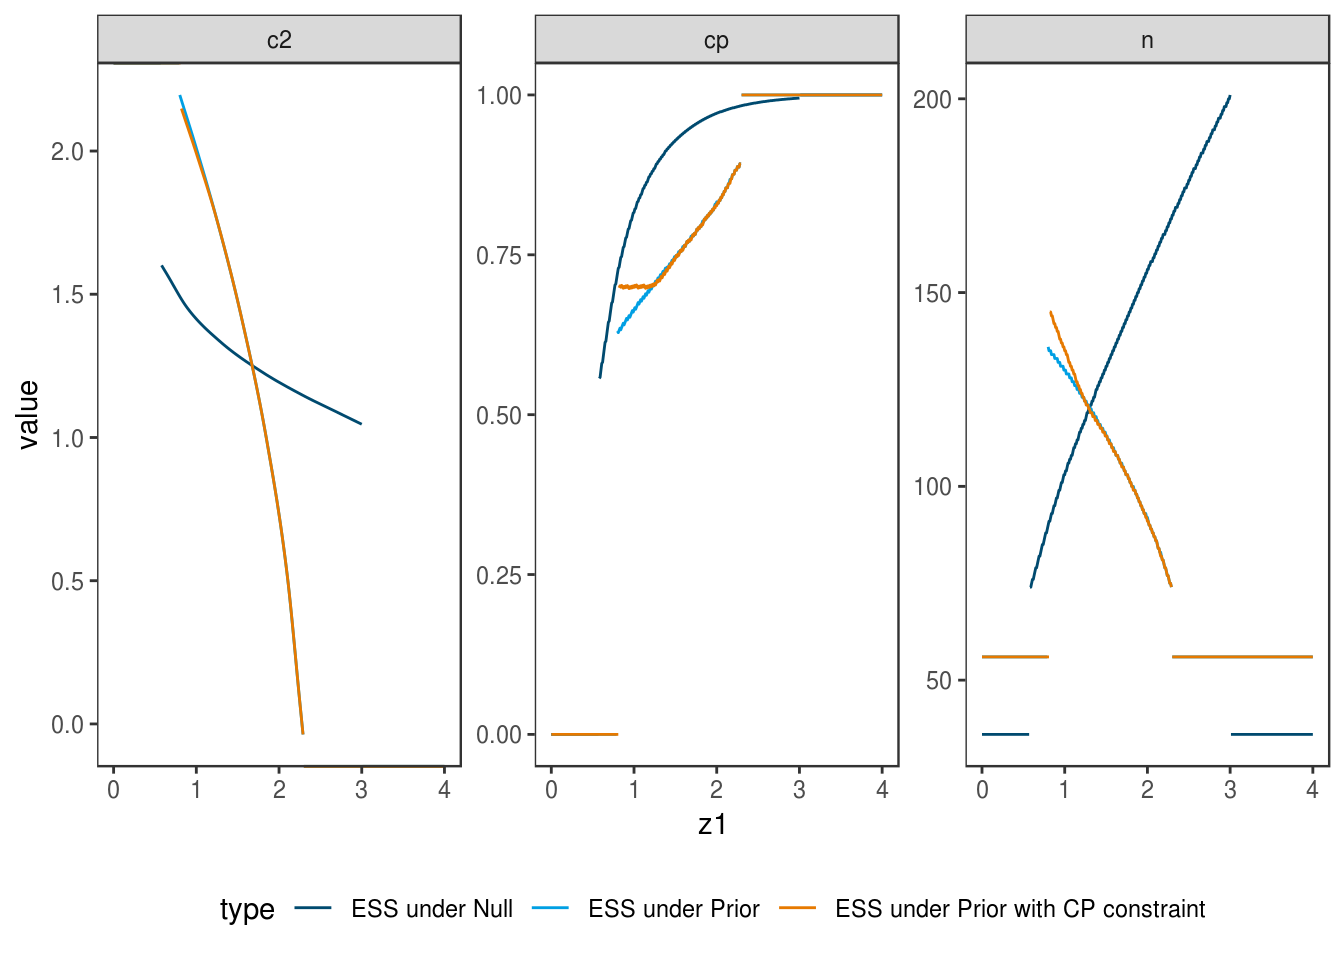
\includegraphics{adoptr-validation-report_files/figure-latex/unnamed-chunk-24-1.pdf}

\bibliography{book.bib,packages.bib}


\end{document}
